\documentclass[a4paper,11pt]{article}
\usepackage[dvipsnames,table]{xcolor}
\usepackage[a4paper,margin=2.5cm,headheight=15pt]{geometry}
\usepackage[utf8]{inputenc}
\usepackage[T1]{fontenc}
\usepackage[serbian]{babel}
\usepackage{lmodern,microtype}
\usepackage{amsmath,amssymb,mathtools}
\numberwithin{equation}{section}
\usepackage{graphicx,adjustbox,placeins}
\graphicspath{{Images/}}
\usepackage{booktabs,tabularx,longtable,array,multirow,makecell}
\usepackage{caption,subcaption}
\captionsetup{font=small,labelfont=bf}
\usepackage{siunitx}
\sisetup{detect-all}
\usepackage[most]{tcolorbox}
\usepackage{enumitem}
\setlist{nosep}
\usepackage{fancyhdr}
\definecolor{Primary}{HTML}{1F77B4}
\definecolor{Accent}{HTML}{2CA02C}
\usepackage[colorlinks=true,linkcolor=Primary,citecolor=Primary,urlcolor=Primary]{hyperref}
\usepackage{cleveref}
\pagestyle{fancy}
\fancyhf{}
\lhead{\small\textit{Analiza logičkih kola sa MOS tranzistorima}}
\rhead{\thepage}
\renewcommand{\arraystretch}{1.25}
\newcolumntype{C}{>{\centering\arraybackslash}X}
\renewcommand{\contentsname}{Sadržaj}
\setlength{\emergencystretch}{2em}
\allowdisplaybreaks[2]
\newcommand{\napomena}[1]{\begin{tcolorbox}[colback=gray!10,colframe=black,boxrule=0.5pt,breakable]#1\end{tcolorbox}}
\newcommand{\redlinija}{\arrayrulecolor{black!28}\specialrule{0.3pt}{2pt}{2pt}\arrayrulecolor{black}}
\newcommand{\kod}[1]{\ensuremath{\mathtt{#1}}}
\begin{document}
\hypersetup{pageanchor=false}
\begin{titlepage}
\thispagestyle{empty}
\begin{center}
{\Large\bfseries UNIVERZITET U BEOGRADU -- ELEKTROTEHNIČKI FAKULTET\\ KATEDRA ZA ELEKTRONIKU\par}
\vspace{25mm}
{\LARGE\bfseries DIGITALNA ELEKTRONIKA 1\par}
\vspace{2mm}
{\large Materijali za računske vežbe\par}
\vspace{18mm}
{\Large\bfseries ANALIZA LOGIČKIH KOLA SA MOS TRANZISTORIMA\par}
\vspace{3mm}
{\large Vežbe 8\par}
\vfill
\begin{minipage}{0.62\linewidth}
\raggedright\textbf{Autori:}\\[4pt]\small
\begin{tabular}{@{}ll@{}}
Nikola Petrović & \href{mailto:p.z.nikola@etf.bg.ac.rs}{\texttt{p.z.nikola@etf.bg.ac.rs}}\\
Haris Turkmanović & \href{mailto:haris@etf.bg.ac.rs}{\texttt{haris@etf.bg.ac.rs}}\\
\end{tabular}
\end{minipage}\hfill
\begin{minipage}{0.34\linewidth}\raggedleft Beograd, \today\end{minipage}
\end{center}
\end{titlepage}
\hypersetup{pageanchor=true}
\tableofcontents
\newpage
\section*{Modeli i oznake}\addcontentsline{toc}{section}{Modeli i oznake}
Koristimo pojednostavljeni model izvornika, bez modulacije dužine kanala, struja curenja i parazitskih kapacitivnosti, osim gde su izričito potrebne. Za NMOS označimo $B=\mu_nC_{ox}W/L$, $E=E_C L$ i $u=V_{GS}-V_T$. Struje u omskoj oblasti i zasićenju su
\begin{equation}\label{eq:model}
I_{D,\mathrm{lin}}=\frac{B}{1+V_{DS}/E}\left(uV_{DS}-\frac{V_{DS}^2}{2}\right),\qquad I_{D,\mathrm{sat}}=\frac{B}{2}\frac{u^2}{1+u/E}.
\end{equation}

U ovom modelu granica oblasti uzima se kao $V_{DS}=u$, a $v_{\mathrm{sat}}=\mu_nE_C/2$. Model je aproksimacija efekata kratkog kanala; nije zamena za model konkretne tehnologije. Za $V_{DS}/E\ll1$, odnosno $u/E\ll1$, odgovarajući imenilac može se aproksimirati jedinicom. Za PMOS se koriste pozitivni naponi $V_{SG},V_{SD}$ i prag $|V_{TP}|$.
Kao u vežbi 07, $V_H,V_L$ označavaju krajnje/stabilne nivoe bez poremećaja; garantovane granice su $V_{OH}=f(V_{IL})$ i $V_{OL}=f(V_{IH})$. Izvor često označava $V_H,V_L$ simbolima $V_{OH},V_{OL}$ i njima aproksimira garantovane nivoe. Ta aproksimacija ovde je posebno naznačena.
\section{Zadatak 1: NMOS invertor sa pasivnim opterećenjem}\label{sec:1}
\begin{enumerate}[label=\alph*)]
\item Za NMOS invertor sa kratkim kanalom i otpornim opterećenjem odrediti izraze za izlazne nivoe, $V_{IL},V_{IH}$ i napon prebacivanja $V_S$.
\item Izračunati margine šuma za višestruke izvore šuma ako je $\mu_n C_{ox}=430\,\mathrm{\mu A/V^2}$, $V_T=0.4\,\mathrm V$, $W/L=2$, $V_{DD}=1.2\,\mathrm V$, $R_L=20\,\mathrm{k\Omega}$.
\end{enumerate}
\begin{figure}[!htbp]\centering
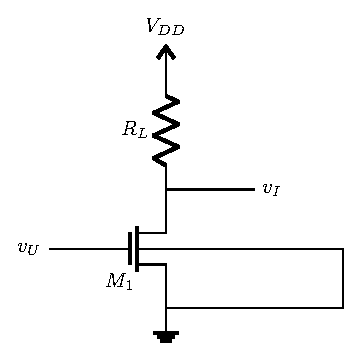
\includegraphics[width=.45\linewidth,height=.36\textheight,keepaspectratio]{Zadatak_1/invertor}
\caption{NMOS invertor sa otpornim opterećenjem; podloga je vezana za masu.}\label{fig:1.1}
\end{figure}
\subsection*{Rešenje}
\paragraph{a) Izlazni nivoi i pragovi.}
Za $v_U<V_T$ tranzistor ne vodi, pa nema pada napona na otporniku i $V_H=V_{DD}$. Kada je ulaz $V_H$, izlaz $V_L$ je nizak, a tranzistor u omskoj oblasti. Iz $I_{R_L}=I_D$ sledi
\begin{equation}\label{eq:1.1}
\frac{V_{DD}-V_L}{R_L}=\frac{B_n}{1+V_L/E}\left[(V_H-V_T)V_L-\frac{V_L^2}{2}\right].
\end{equation}

Ako se zanemari $V_L/E$, dobija se, uz $\alpha=1/(B_nR_L)$,
\begin{equation}\label{eq:1.9}
V_L^2-2(\alpha+V_{DD}-V_T)V_L+2\alpha V_{DD}=0.
\end{equation}

Bira se manji koren koji zadovoljava $0\le V_L<V_{DD}-V_T$, a ne proizvoljan pozitivan koren. Zanemarivanjem i $V_L^2$ dobija se dodatna aproksimacija
\begin{equation}\label{eq:1.10}
V_L\approx\frac{V_{DD}}{1+B_nR_L(V_{DD}-V_T)}.
\end{equation}

Ulazne granice su tačke nagiba $\mathrm d v_I/\mathrm d v_U=-1$. Blizu $V_{IL}$ tranzistor radi u zasićenju:
\begin{equation}\label{eq:1.2}
\frac{V_{DD}-v_I}{R_L}=\frac{B_n}{2}\frac{(v_U-V_T)^2}{1+(v_U-V_T)/E}=\frac{Wv_{\mathrm{sat}}C_{ox}(v_U-V_T)^2}{(v_U-V_T)+E}.
\end{equation}

Ako je $(v_U-V_T)/E\ll1$, tada
\begin{equation}\label{eq:1.3}
\frac{V_{DD}-v_I}{R_L}\approx\frac{B_n}{2}(v_U-V_T)^2,
\end{equation}
\begin{equation}\label{eq:1.4}
-\frac1{R_L}\frac{\mathrm d v_I}{\mathrm d v_U}=B_n(v_U-V_T),\qquad V_{IL}=V_T+\alpha.
\end{equation}

Blizu $V_{IH}$ tranzistor je u omskoj oblasti:
\begin{equation}\label{eq:1.5}
\frac{V_{DD}-v_I}{R_L}=\frac{B_n}{1+v_I/E}\left[(v_U-V_T)v_I-\frac{v_I^2}{2}\right].
\end{equation}
\begin{equation}\label{eq:1.6}
\frac{V_{DD}-v_I}{R_L}\approx B_n\left[(v_U-V_T)v_I-\frac{v_I^2}{2}\right].
\end{equation}

Diferenciranje daje $-v_I'/R_L=B_n[(v_U-V_T)v_I'+v_I-v_Iv_I']$. U tački $v_I'=-1$:
\begin{equation}\label{eq:1.7}
\frac1{R_L}=B_n(V_T-V_{IH}+2v_I),\qquad V_{IH}=V_T-\alpha+\sqrt{\frac{8\alpha V_{DD}}3}.
\end{equation}

Na pragu $v_U=v_I=V_S$, NMOS je u zasićenju ($V_{DG}=0$), pa
\begin{equation}\label{eq:1.8}
\frac{V_{DD}-V_S}{R_L}=\frac{B_n}{2}\frac{(V_S-V_T)^2}{1+(V_S-V_T)/E}.
\end{equation}

Može se rešavati numerički na fizičkom intervalu $(V_T,V_{DD})$, npr. bisekcijom. Početna procena $V_{DD}/2$ nije dodatna jednačina.
\paragraph{b) Numerički rezultati.}
$B_n=860\,\mathrm{\mu A/V^2}$ i $\alpha=0.0581395\,\mathrm V$. U aproksimaciji bez korekcije kratkog kanala:
\begin{center}\begin{tabular}{lc}\toprule
Veličina & Vrednost\\
\midrule
$V_H$ & $1.2\,\mathrm V$\\
\redlinija
$V_L$, dodatno linearizovano & $0.081301\,\mathrm V$\\
\redlinija
$V_L$, manji koren kvadratne jednačine & $0.085567\,\mathrm V$\\
\redlinija
$V_{IL}$ & $0.458140\,\mathrm V$\\
\redlinija
$V_{IH}$ & $0.773192\,\mathrm V$\\
\bottomrule\end{tabular}\end{center}
Procene margina pomoću krajnjih nivoa iz izvornika su $NM_0\approx0.376839\,\mathrm V\approx0.38\,\mathrm V$ i $NM_1\approx0.426808\,\mathrm V\approx0.43\,\mathrm V$. Ako se garantovani izlazi odrede u tačkama nagiba $-1$ u istom aproksimativnom modelu, sledi
\begin{equation}\label{eq:1.11}
\begin{aligned}V_{OH}&=V_{DD}-\alpha/2=1.170930\,\mathrm V,\\ V_{OL}&=\sqrt{2\alpha V_{DD}/3}=0.215666\,\mathrm V,\\ NM_0&=0.242474\,\mathrm V,\qquad NM_1=0.397739\,\mathrm V.\end{aligned}
\end{equation}

\napomena{Parametar $E_C L$ nije zadat. Zato se iz datih podataka ne mogu izračunati tačni rezultati modela kratkog kanala niti potvrditi mala vrednost zanemarenih odnosa. Bez tih korekcija dobilo bi se $V_S=0.652350\,\mathrm V$; to je samo rezultat označene aproksimacije.}
\FloatBarrier\section{Zadatak 2: opterećenje sa indukovanim kanalom}\label{sec:2}
\begin{enumerate}[label=\alph*)]
\item Za invertor sa slike~\ref{fig:2.1} odrediti visoki izlazni nivo i $K_R=(W_1/L_1)/(W_2/L_2)$. Dato je $2|\phi_F|=0.88\,\mathrm V$, $V_{T0}=0.4\,\mathrm V$, $V_{DD}=1.2\,\mathrm V$, $\gamma=0.2\,\mathrm{V^{1/2}}$, $\mu_n=270\,\mathrm{cm^2/(Vs)}$, $C_{ox}=1.6\,\mathrm{\mu F/cm^2}$, $v_{\mathrm{sat}}=8.0\cdot10^6\,\mathrm{cm/s}$, $E_CL=0.6\,\mathrm V$, $V_L=0.1\,\mathrm V$, $L_1=L_2=100\,\mathrm{nm}$ i $V_{GG}=V_{DD}$.
\item Odrediti donju granicu napona $V_{GG}$ za omski rad opteretnog tranzistora u celom opsegu izlaza, kao i visoki izlazni nivo u tom slučaju.
\end{enumerate}
\begin{figure}[!htbp]\centering

\includegraphics[width=.5\linewidth,height=.36\textheight,keepaspectratio]{Zadatak_2/invertor}
\caption{NMOS invertor sa opteretnim tranzistorom sa indukovanim kanalom.}\label{fig:2.1}
\end{figure}
\subsection*{Rešenje}
\paragraph{a) Efekat podloge i odnos geometrija.}
Za $V_{GG}=V_{DD}$ opteretni tranzistor ima spojene gejt i drejn, pa kada vodi radi u zasićenju. Punjenje izlaza prestaje pri $V_H=V_{DD}-V_{T2}(V_H)$. Pošto su podloge na masi,
\begin{equation}\label{eq:2.4}
V_{T2}(v)=V_{T0}+\gamma\left(\sqrt{v+2|\phi_F|}-\sqrt{2|\phi_F|}\right).
\end{equation}
\begin{equation}\label{eq:2.1}
V_H=V_{DD}-V_{T0}-\gamma\left(\sqrt{V_H+2|\phi_F|}-\sqrt{2|\phi_F|}\right).
\end{equation}

Kada se naponi izraze u voltima, numerička jednačina je $V_H=0.9876166-0.2\sqrt{V_H+0.88}$. Iteracija počev od $0.8$ daje $V_H=0.733564\,\mathrm V$; efekat podloge smanjuje izlazni visoki nivo.
Na niskom izlazu $v_I=V_L$, sa ulazom $v_U=V_H$, $M_1$ radi omski, a $M_2$ u zasićenju. Jednakost struja je
\begin{equation}\label{eq:2.2}
\frac{W_1\mu_nC_{ox}}{L_1(1+v_I/E_1)}\left[(v_U-V_{T1})v_I-\frac{v_I^2}{2}\right]=\frac{W_2v_{\mathrm{sat}}C_{ox}(V_{DD}-v_I-V_{T2})^2}{V_{DD}-v_I-V_{T2}+E_2}.
\end{equation}

Ovde je $V_{T1}=V_{T0}$ i $V_{T2}(0.1\,\mathrm V)=0.410373\,\mathrm V$. Obe pretpostavljene oblasti rada su zadovoljene: $0.1<0.733564-0.4$, a $V_{DS2}=V_{GS2}=1.1\,\mathrm V$. Uz $u_2=V_{DD}-V_L-V_{T2}(V_L)$,
\begin{equation}\label{eq:2.5}
K_R=\frac{v_{\mathrm{sat}}L_2}{\mu_n}\,\frac{(1+V_L/E_1)u_2^2}{(u_2+E_2)[(V_H-V_{T0})V_L-V_L^2/2]}\approx4.49558.
\end{equation}

\napomena{Broj $1.7$ u izvorniku ne zadovoljava datu jednačinu struja. Dati parametri su blago neusaglašeni: $2v_{\mathrm{sat}}L/\mu_n=0.592593\,\mathrm V$, dok je zadato $E_CL=0.6\,\mathrm V$. Direktna upotreba datih brojeva u~\eqref{eq:2.2} daje $K_R=4.49558$. Ako se nametne tačna relacija $v_{\mathrm{sat}}=\mu_nE_C/2$ uz $E_CL=0.6\,\mathrm V$, dobija se $K_R=4.55177$. Razlika je oko 1.25\%, pa su oba jasno označena tumačenja navedena.}
\paragraph{b) Povišeno upravljanje opterećenjem.}
Uslov omskog rada je $V_{DS2}<V_{GS2}-V_{T2}$, odnosno
\begin{equation}\label{eq:2.3}
V_{GG}>V_{DD}+\max_{0\le v_I\le V_{DD}}V_{T2}(v_I)=V_{DD}+V_{T2}(V_{DD}).
\end{equation}

Prag raste sa naponom sorsa, pa maksimum nastupa na $V_{DD}$. Dobijamo $V_{T2}(V_{DD})=0.500827\,\mathrm V$ i $V_{GG}>1.700827\,\mathrm V$. Broj $1.700827\,\mathrm V$ je donja granica (infimum); za strogu nejednakost ne postoji najmanja dopuštena vrednost. Visoki izlaz tada teži $V_H=V_{DD}=1.2\,\mathrm V$ u idealnom statičkom modelu.
\FloatBarrier\section{Zadatak 3: opterećenje sa ugrađenim kanalom}\label{sec:3}
Za NMOS invertor sa slike~\ref{fig:3.1}, čije opterećenje ima ugrađeni kanal i kratko spojene gejt i sors, odrediti margine šuma za višestruke izvore šuma.
\begin{figure}[!htbp]\centering

\includegraphics[width=.6\linewidth,height=.36\textheight,keepaspectratio]{Zadatak_3/invertor}
\caption{Invertor sa opteretnim tranzistorom sa ugrađenim kanalom.}\label{fig:3.1}
\end{figure}
\subsection*{Rešenje}
Za $M_2$ je $V_{T02}<0$, pa kanal postoji i pri $V_{GS2}=0$. Zasićenje nastupa kada $V_{DS2}\ge -V_{T2}=|V_{T2}|$. Efekat podloge daje
\begin{equation}\label{eq:3.9}
V_{T2}(v_I)=V_{T02}+\gamma\left(\sqrt{v_I+2|\phi_F|}-\sqrt{2|\phi_F|}\right).
\end{equation}

Pretpostavlja se da $V_{T2}(v_I)<0$ u celom posmatranom opsegu. Inače opterećenje može prestati da vodi pre dostizanja šine i analiza se mora prilagoditi. Kada je $M_1$ isključen, $M_2$ je pri kraju punjenja u omskoj oblasti i $V_H=V_{DD}$, a ne unapred zadatih $5\,\mathrm V$.
\paragraph{Određivanje $V_{IL}$.}
$M_1$ je u zasićenju, a $M_2$ omski. Uz $t(v_I)=-V_{T2}(v_I)>0$ i $d=V_{DD}-v_I$, jednakost struja je
\begin{equation}\label{eq:3.1}
\frac{W_1v_{\mathrm{sat}}C_{ox}(v_U-V_{T1})^2}{v_U-V_{T1}+E_1}=\frac{W_2\mu_nC_{ox}}{L_2(1+d/E_2)}\left[t(v_I)d-\frac{d^2}{2}\right].
\end{equation}

Za male $(v_U-V_{T1})/E_1$ i $d/E_2$, a uz privremeno konstantan $t=t(V_{DD})$, važi
\begin{equation}\label{eq:3.2}
\frac{W_1v_{\mathrm{sat}}C_{ox}}{E_1}(v_U-V_{T1})^2\approx\frac{W_2\mu_nC_{ox}}{L_2}\left[td-\frac{d^2}{2}\right],
\end{equation}
\begin{equation}\label{eq:3.3}
K_R(v_U-V_{T1})^2=2td-d^2,\qquad K_R=\frac{W_1L_2}{W_2L_1}.
\end{equation}

Diferenciranjem i postavljanjem $v_I'=-1$ dobijamo
\begin{equation}\label{eq:3.4}
v_I=V_{DD}-t+K_R(V_{IL}-V_{T1}).
\end{equation}

Sistem~\eqref{eq:3.3}–\eqref{eq:3.4} daje
\begin{equation}\label{eq:3.10}
V_{IL}=V_{T1}+\frac{t}{\sqrt{K_R(K_R+1)}},\qquad V_{OH}\approx V_{DD}-t\left(1-\sqrt{\frac{K_R}{K_R+1}}\right).
\end{equation}

Ako se efekat podloge ne zamrzne na referentnoj tački, pri diferenciranju mora se uključiti $\mathrm d t/\mathrm d v_I$; prethodni zatvoreni izrazi tada ne važe.
\paragraph{Određivanje $V_{IH}$ i niskog nivoa.}
Sada je $M_1$ omski, a $M_2$ u zasićenju:
\begin{equation}\label{eq:3.5}
\frac{W_1\mu_nC_{ox}}{L_1(1+v_I/E_1)}\left[(v_U-V_{T1})v_I-\frac{v_I^2}{2}\right]=\frac{W_2v_{\mathrm{sat}}C_{ox}\,t(v_I)^2}{t(v_I)+E_2}.
\end{equation}

Uz $v_I/E_1\ll1$ i konstantan $t_0=-V_{T02}$, definišimo $Q=t_0^2/(1+t_0/E_2)>0$. Tada
\begin{equation}\label{eq:3.6}
K_R[2(v_U-V_{T1})v_I-v_I^2]=Q,
\end{equation}
\begin{equation}\label{eq:3.7}
V_{IH}-V_{T1}=2v_I,\qquad V_{OL}\approx\sqrt{\frac{Q}{3K_R}},\qquad V_{IH}=V_{T1}+2\sqrt{\frac{Q}{3K_R}}.
\end{equation}

Na krajnjem niskom nivou ($v_U=V_H$) sledi
\begin{equation}\label{eq:3.8}
K_R[2(V_H-V_{T1})V_L-V_L^2]=Q.
\end{equation}

Manji fizički koren je $V_L=(V_H-V_{T1})-\sqrt{(V_H-V_{T1})^2-Q/K_R}$. Ako se zanemari $V_L^2$, $V_L\approx Q/[2K_R(V_H-V_{T1})]$.
Garantovane margine u navedenoj aproksimaciji su $NM_0=V_{IL}-V_{OL}$ i $NM_1=V_{OH}-V_{IH}$. Izvorna procena zamenjuje $V_{OL},V_{OH}$ krajnjim nivoima $V_L,V_H$.
\napomena{Nisu dati napajanje, geometrije ni parametri tranzistora. Zato se ne mogu navesti jedinstvene numeričke margine. Svako simboličko rešenje zahteva nenegativan diskriminant, napone između šina i proveru pretpostavljenih oblasti rada.}
\FloatBarrier\section{Zadatak 4: CMOS invertor}\label{sec:4}
\begin{enumerate}[label=\alph*)]
\item U ravni $(v_U,v_I)$ odrediti oblasti rada NMOS i PMOS tranzistora CMOS invertora (\emph{Complementary MOS}).
\item Izračunati $V_S$ za $W_{p1}=400\,\mathrm{nm}$ i $W_{p2}=100\,\mathrm{nm}$, uz $W_n=100\,\mathrm{nm}$ i $L_n=L_p=100\,\mathrm{nm}$. Dato je $V_{DD}=1.2\,\mathrm V$, $V_{TN}=|V_{TP}|=0.4\,\mathrm V$, $E_{CP}=24\,\mathrm{V/\mu m}=4E_{CN}$. Objasniti uticaj širine PMOS tranzistora.
\end{enumerate}
\subsection*{Rešenje}
\paragraph{a) Oblasti rada.}
NMOS vodi ako je $v_U>V_{TN}$, a PMOS ako je $V_{DD}-v_U>|V_{TP}|$. Za tranzistore koji vode:
\begin{equation}\label{eq:4.1}
\begin{aligned}\text{NMOS zasićen:}\quad&v_I\ge v_U-V_{TN},\\\text{PMOS zasićen:}\quad&V_{DD}-v_I\ge V_{DD}-v_U-|V_{TP}|,\\&v_I\le v_U+|V_{TP}|.\end{aligned}
\end{equation}

Suprotne stroge nejednakosti određuju omske oblasti; jednakosti su granice. Isključene oblasti određuju samo uslovi gejta. Na $v_U=v_I=V_S$ oba tranzistora su u zasićenju.
\begin{figure}[!htbp]\centering
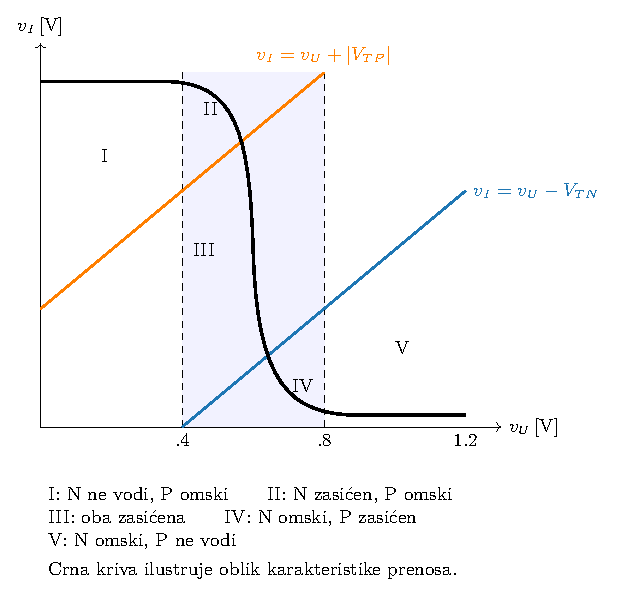
\includegraphics[width=.95\linewidth,height=.36\textheight,keepaspectratio]{Zadatak_4/oblasti}
\caption{Granice oblasti rada: N označava NMOS, P PMOS.}\label{fig:4.1}
\end{figure}
\paragraph{b) Napon prebacivanja.}
Uz pretpostavku istog $v_{\mathrm{sat}}$ i $C_{ox}$ za oba tipa, koju koristi i izvor, izjednačavaju se struje:
\begin{equation}\label{eq:4.2}
\frac{W_n(V_S-V_{TN})^2}{V_S-V_{TN}+E_{CN}L_n}=\frac{W_p(V_{DD}-V_S-|V_{TP}|)^2}{V_{DD}-V_S-|V_{TP}|+E_{CP}L_p}.
\end{equation}

$E_{CN}=6\,\mathrm{V/\mu m}$, pa $E_{CN}L_n=0.6\,\mathrm V$, a $E_{CP}L_p=2.4\,\mathrm V$. Rešavanje bez zamrzavanja imenilaca daje
\begin{center}\begin{tabular}{ccc}\toprule
$W_p\,[\mathrm{nm}]$ & $W_p/W_n$ & $V_S\,[\mathrm V]$\\
\midrule
400 & 4 & 0.611288\\
\redlinija
100 & 1 & 0.537965\\
\bottomrule\end{tabular}\end{center}
Rešenja su u intervalu $(0.4,0.8)\,\mathrm V$ i zadovoljavaju pretpostavljene oblasti rada. Jači PMOS pomera prag naviše: potreban je viši ulaz da NMOS uravnoteži njegovu struju.
U izvorniku se zanemaruje prenapon u PMOS imeniocu i NMOS imenilac zamenjuje konstantom; ovde za to nema potrebe. Ako brzine zasićenja ili oksidne kapacitivnosti nisu jednake, njihov odnos mora ostati u~\eqref{eq:4.2}; bez njega prag nije jednoznačno zadat.
\FloatBarrier\section{Zadatak 5: sinteza statičkog CMOS kola}\label{sec:5}
\begin{enumerate}[label=\alph*)]
\item Realizovati $Y=(A+B)(C+D)$ jednostepenim statičkim CMOS kolom ako su negacije ulaza raspoložive.
\item Realizovati istu funkciju najmanjim brojem tranzistora u komplementarnoj statičkoj CMOS realizaciji kada negacije ulaza nisu raspoložive.
\end{enumerate}
\subsection*{Rešenje}
\paragraph{a) Raspoloživi komplementarni ulazi.}
PDN (\emph{pull-down network}) povezuje izlaz sa masom kada je $Y=0$. Zato
\begin{equation}\label{eq:5.1}
\bar Y=\overline{(A+B)(C+D)}=\bar A\bar B+\bar C\bar D.
\end{equation}

Proizvodu odgovara redna, a zbiru paralelna veza NMOS tranzistora. PUN (\emph{pull-up network}) je dualna mreža PMOS tranzistora: serijske veze prelaze u paralelne i obratno, uz iste signale na gejtovima. PMOS provodi za nulu na gejtu. Dobija se ukupno osam tranzistora.
\begin{figure}[!htbp]\centering
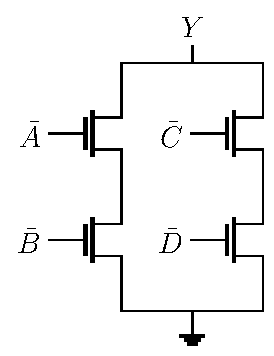
\includegraphics[width=.4\linewidth,height=.36\textheight,keepaspectratio]{Zadatak_5/pdn}
\caption{PDN za funkciju iz tačke a).}\label{fig:5.1}
\end{figure}\begin{figure}[!htbp]\centering
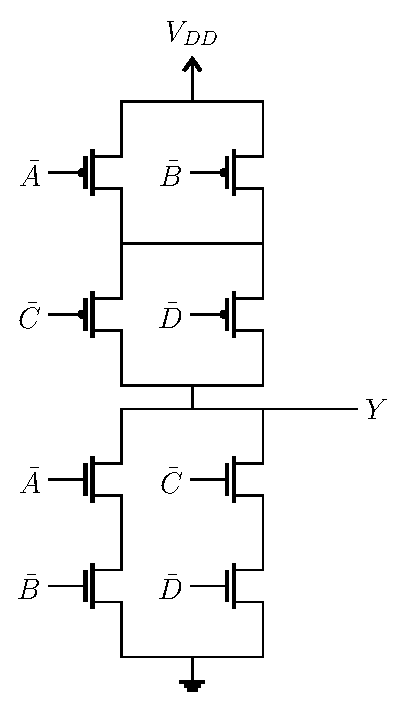
\includegraphics[width=.48\linewidth,height=.36\textheight,keepaspectratio]{Zadatak_5/cmos}
\caption{Kompletna komplementarna CMOS realizacija.}\label{fig:5.2}
\end{figure}
\paragraph{b) Samo direktni ulazi.}
Prvo se realizuje $Y_1=\overline{(A+B)(C+D)}$ pomoću osam tranzistora, pa se doda izlazni CMOS invertor sa dva tranzistora. Ukupno je potrebno deset tranzistora. Četiri zasebna ulazna invertora uz realizaciju iz a) zahtevala bi šesnaest. Minimalnost se ovde odnosi na uobičajene komplementarne statičke CMOS mreže; nije tvrdnja o svim tranzistorskim porodicama.
\begin{figure}[!htbp]\centering
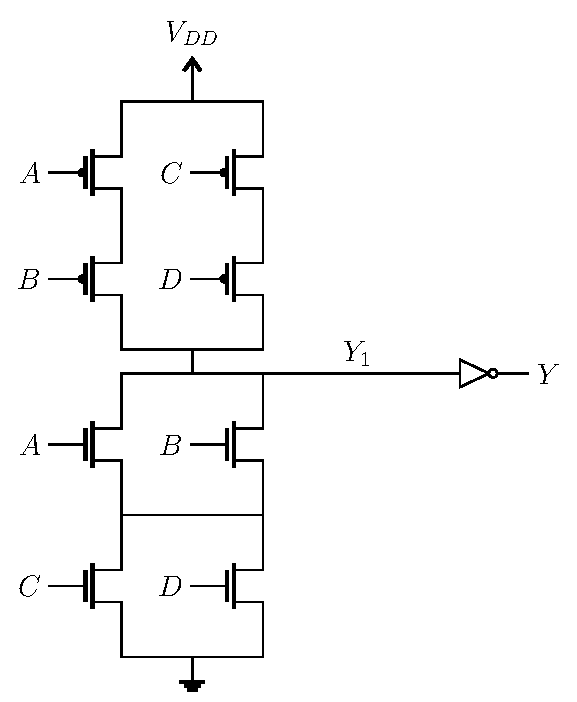
\includegraphics[width=.65\linewidth,height=.36\textheight,keepaspectratio]{Zadatak_5/bez_negacija}
\caption{Realizacija sa direktnim ulazima i završnim invertorom.}\label{fig:5.3}
\end{figure}
\FloatBarrier\section{Zadatak 6: dualne PDN i PUN mreže}\label{sec:6}
Za PDN sa slike~\ref{fig:6.1}: a) odrediti funkciju; b) nacrtati kompletno statičko CMOS kolo.
\begin{figure}[!htbp]\centering

\includegraphics[width=.5\linewidth,height=.36\textheight,keepaspectratio]{Zadatak_6/pdn}
\caption{Zadata PDN mreža.}\label{fig:6.1}
\end{figure}
\subsection*{Rešenje}
\paragraph{a) Logička funkcija.}
\begin{equation}\label{eq:6.1}
\bar Y=A+B(C+D),\qquad Y=\overline{A+B(C+D)}=\bar A\bar B+\bar A\bar C\bar D.
\end{equation}

\paragraph{b) Konstrukcija dualne mreže.}
PM1 je tranzistor $A$, a PM2 ostatak mreže. U PDN su paralelni, pa su u PUN redni. U PM2 je PM3 tranzistor $B$, a PM4 grupa $C,D$. U PDN su PM3 i PM4 redni, pa su u PUN paralelni. PM4 čine PM5 ($C$) i PM6 ($D$): oni su paralelni u PDN, a redni u PUN. Hijerarhija je prikazana na slici~\ref{fig:6.2}, a tranzistorska realizacija na slici~\ref{fig:6.3}.
\begin{figure}[!htbp]\centering
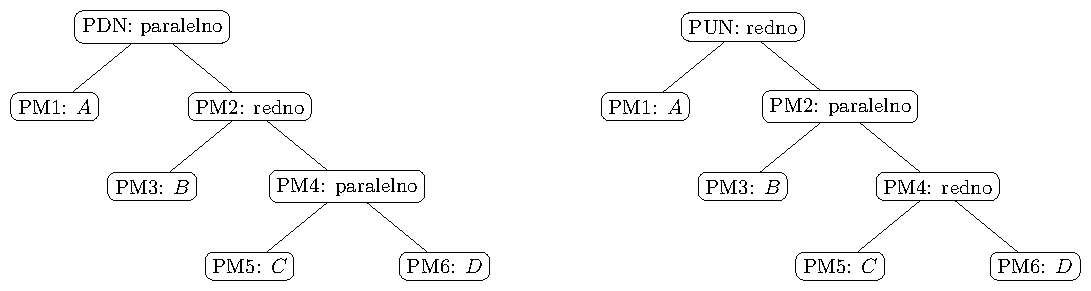
\includegraphics[width=\linewidth,height=.36\textheight,keepaspectratio]{Zadatak_6/dualnost}
\caption{Razlaganje PDN i PUN na iste podmreže sa dualnim vezama.}\label{fig:6.2}
\end{figure}\begin{figure}[!htbp]\centering

\includegraphics[width=.55\linewidth,height=.36\textheight,keepaspectratio]{Zadatak_6/cmos}
\caption{Kompletno statičko CMOS kolo.}\label{fig:6.3}
\end{figure}
\FloatBarrier\section{Zadatak 7: dimenzionisanje tranzistora}\label{sec:7}
Odrediti odnose $W/L$ tranzistora kola sa slike~\ref{fig:7.1}. Zanemaruju se kapacitivnosti svih čvorova osim izlaznog i dato je $\mu_n=2\mu_p$.
\begin{figure}[!htbp]\centering

\includegraphics[width=.5\linewidth,height=.36\textheight,keepaspectratio]{Zadatak_7/cmos}
\caption{Kolo koje se dimenzioniše.}\label{fig:7.1}
\end{figure}
\subsection*{Rešenje}
Sama pokretljivost ne određuje apsolutne dimenzije. Kao u izvorniku, uzimamo zajedničku dužinu kanala, referentni invertor sa normalizovanim odnosima $(W/L)_n=1$, $(W/L)_p=2$ i približno izjednačavamo najgore otpornosti provodnih putanja. U nastavku $w$ označava normalizovani odnos $W/L$.
Za isti tip tranzistora $R\propto1/w$. Redna veza daje
\begin{equation}\label{eq:7.1}
\frac1{w_S}=\frac1{w_1}+\frac1{w_2},\qquad w_S=\frac{w_1w_2}{w_1+w_2}.
\end{equation}

Ako oba paralelna tranzistora vode, $w_P=w_1+w_2$. U najgorem slučaju vodi samo jedan, pa
\begin{equation}\label{eq:7.2}
w_{P,\mathrm{worst}}=\min(w_1,w_2).
\end{equation}
\begin{figure}[!htbp]\centering
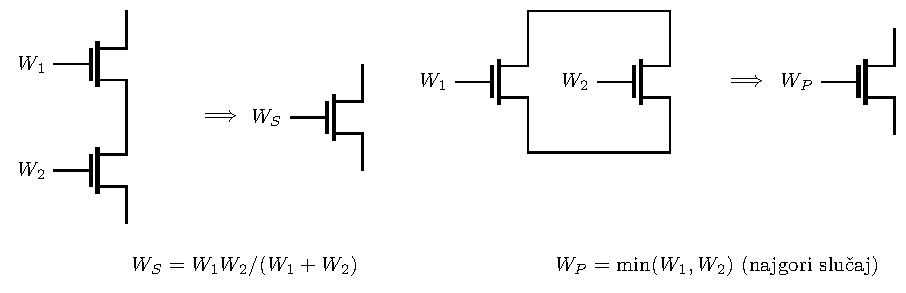
\includegraphics[width=\linewidth,height=.36\textheight,keepaspectratio]{Zadatak_7/ekvivalenti}
\caption{Ekvivalentne širine redne i paralelne veze.}\label{fig:7.2}
\end{figure}
PDN treba da ima najgoru ekvivalentnu širinu 1. Zato je $w_{nA}=1$. Putanje $B$--$C$ i $B$--$D$ imaju po dva redna tranzistora; uz jednaku raspodelu otpornosti uzimamo $w_{nB}=w_{nC}=w_{nD}=2$.
PUN treba da ima najgoru ekvivalentnu širinu 2. Dve redne celine $A$ i $[B\parallel(C+D)]$ dobijaju ekvivalentnu širinu po 4. Zato su $w_{pA}=w_{pB}=4$, a $w_{pC}=w_{pD}=8$. Putanje $A$--$B$ i $A$--$C$--$D$ obe daju $w_{\mathrm{eq}}=2$. Ovo je jedno praktično rešenje, a ne jedinstveno dimenzionisanje bez dodatnog kriterijuma površine ili kašnjenja.
\begin{figure}[!htbp]\centering
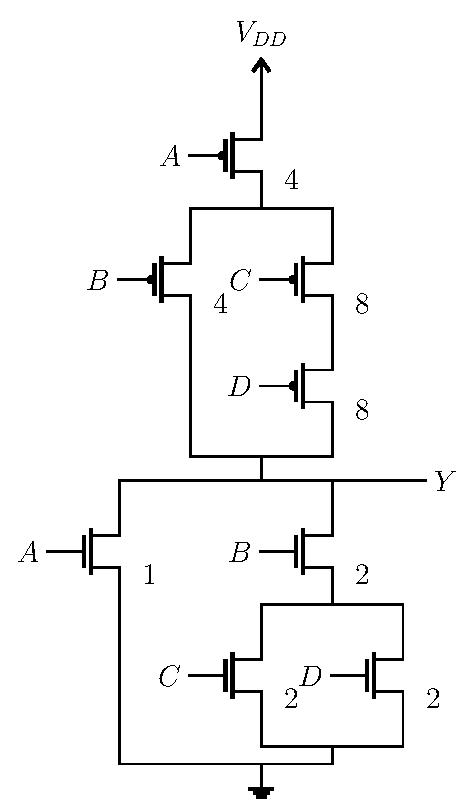
\includegraphics[width=.6\linewidth,height=.36\textheight,keepaspectratio]{Zadatak_7/dimenzije}
\caption{Normalizovani odnosi W/L svih tranzistora.}\label{fig:7.3}
\end{figure}
\FloatBarrier\section{Zadatak 8: dinamička i domino logika}\label{sec:8}
\begin{enumerate}[label=\alph*)]
\item Projektovati jednostepeno dinamičko CMOS kolo za
\[Y=\overline{AB}\left(\overline{\bar C+\bar A\bar D+C(A+D)}+\overline{CD}\right).\]
\item Realizovati $Z=\bar Y$ u domino logici, koristeći CMOS domino I i ILI kola sa proizvoljnim brojem ulaza. Ulazi i njihove negacije su raspoloživi.
\end{enumerate}
\subsection*{Rešenje}
\paragraph{a) Svođenje funkcije.}
Neka je $P=\bar C+\bar A\bar D+C(A+D)$. Za $CD=1$ važi $P=1$, pa $P\,CD=CD$. Otuda
\begin{equation}\label{eq:8.1}
Y=\overline{AB}(\bar P+\overline{CD})=\overline{AB+P\,CD}=\overline{AB+CD}.
\end{equation}

PDN sadrži dve paralelne grane sa po dva redna NMOS tranzistora. PMOS za pretpunjenje i NMOS za evaluaciju upravljani su istim signalom CLK. Za $CLK=0$ izlaz se puni na jedinicu, a za $CLK=1$ može se isprazniti kroz PDN.
\begin{figure}[!htbp]\centering
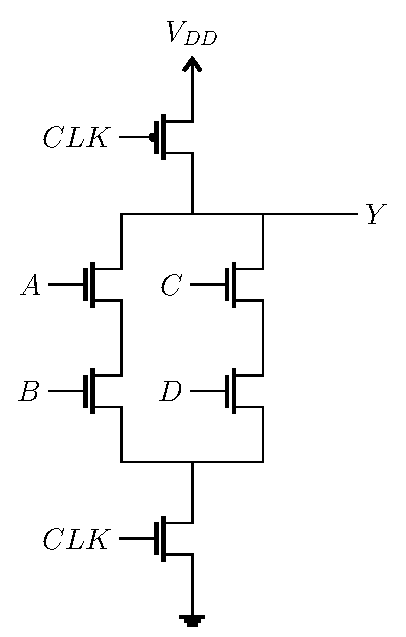
\includegraphics[width=.5\linewidth,height=.36\textheight,keepaspectratio]{Zadatak_8/dinamicko}
\caption{Dinamičko kolo za Y; logička funkcija važi u fazi evaluacije.}\label{fig:8.1}
\end{figure}
\paragraph{b) Domino realizacija.}
\begin{equation}\label{eq:8.2}
Z=\bar Y=AB+CD.
\end{equation}

Na izlazu svakog dinamičkog stepena nalazi se statički invertor. Zato domino I stepeni daju $P=AB$, $Q=CD$, a završni domino ILI daje $Z=P+Q$. Negacije složenih izraza uklanjaju se De Morganovim pravilima $\overline{AB}=\bar A+\bar B$, $\overline{A+B}=\bar A\bar B$.
Raspoloživost negiranih signala sama po sebi ne garantuje ispravan vremenski rad: tokom evaluacije ulazi domino stepena moraju biti stabilni ili monotono prelaziti sa 0 na 1. Izlaz invertora posle pretpunjenja počinje nulom i može samo porasti, što omogućava kaskadiranje. Izbegavaju se padovi koji bi nepovratno ispraznili naredni dinamički čvor.
\begin{figure}[!htbp]\centering
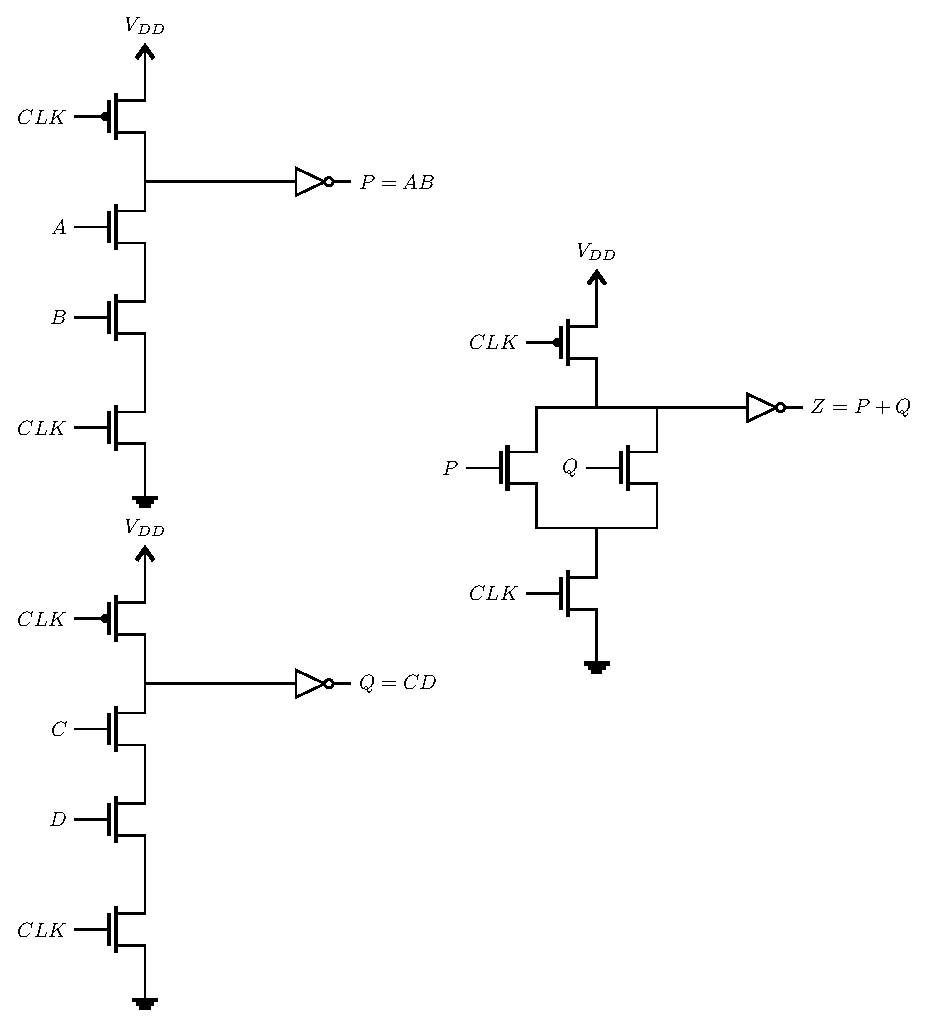
\includegraphics[width=.78\linewidth,height=.60\textheight,keepaspectratio]{Zadatak_8/domino}
\caption{Tri domino stepena; jednako označeni P i Q predstavljaju povezane vodove.}\label{fig:8.2}
\end{figure}
\FloatBarrier\section{Zadatak 9: vremenski dijagram dinamičkog kola}\label{sec:9}
Za dato dinamičko kolo i ulazne signale sa slika~\ref{fig:9.1} i~\ref{fig:9.inputs} nacrtati izlaz $Y(t)$.
\begin{figure}[!htbp]\centering

\includegraphics[width=.4\linewidth,height=.36\textheight,keepaspectratio]{Zadatak_9/kolo}
\caption{Dinamičko kolo sa PDN funkcijom C(A+B).}\label{fig:9.1}
\end{figure}\begin{figure}[!htbp]\centering
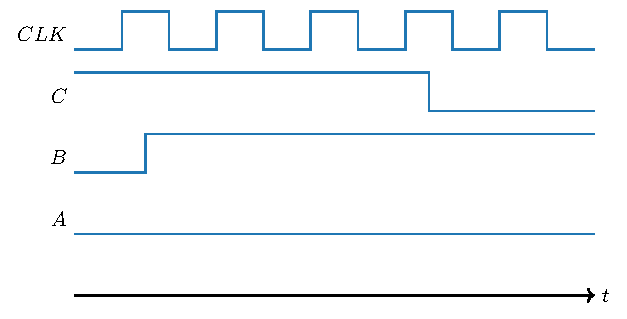
\includegraphics[width=.9\linewidth,height=.36\textheight,keepaspectratio]{Zadatak_9/ulazi}
\caption{Zadati ulazi; vremenska osa je relativna, bez zadatih numeričkih trajanja.}\label{fig:9.inputs}
\end{figure}
\subsection*{Rešenje}
U fazi evaluacije ostvaruje se $Y=\overline{C(A+B)}$, uz pamćenje prethodnog pražnjenja. Dok je $CLK=0$, PMOS puni čvor i $Y=1$. Dok je $CLK=1$, izlaz može preći sa 1 na 0 kada postoji provodna putanja prema masi, ali ne može ponovo porasti pre sledećeg pretpunjenja.
Na uzlaznoj ivici $B$ u prvoj fazi evaluacije važi $C=1$, pa izlaz pada na 0. Sledeće pretpunjenje ga vraća na 1. U narednim fazama sa $B=C=1$ izlaz ponovo pada. Kada $C$ opadne usred evaluacije, putanja ka masi se prekida, ali već ispražnjeni čvor ostaje na 0 do prvog narednog $CLK=0$. Posle toga, dok je $C=0$, izlaz ostaje visok. Zanemarena su propagaciona kašnjenja, curenje i raspodela naelektrisanja.
\begin{figure}[!htbp]\centering
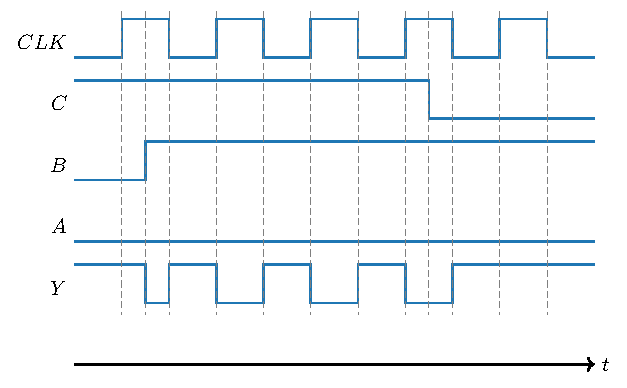
\includegraphics[width=.9\linewidth,height=.36\textheight,keepaspectratio]{Zadatak_9/izlaz}
\caption{Izlaz pamti pražnjenje do sledeće faze pretpunjenja.}\label{fig:9.2}
\end{figure}
\FloatBarrier\section{Zadatak 10: transmisioni gejtovi}\label{sec:10}
\begin{enumerate}[label=\alph*)]
\item Odrediti funkcionalnu tabelu kola sa slike~\ref{fig:10.1} za binarne ulaze.
\item Dopuniti opis kada $D$ može biti u stanju visoke impedanse.
\item Transmisionim gejtovima realizovati $Y=AC+BC$.
\end{enumerate}
Transmisioni gejt (TG) je paralelna veza NMOS i PMOS prekidača sa komplementarnim upravljanjem. Gornja oznaka u simbolu je upravljanje NMOS-om; TG provodi kada je ona 1, dok PMOS dobija njen komplement. Jednako označeni vodovi su povezani. Podrazumevaju se raspoloživi komplementarni upravljački signali i idealan statički model prekidača.
\begin{figure}[!htbp]\centering
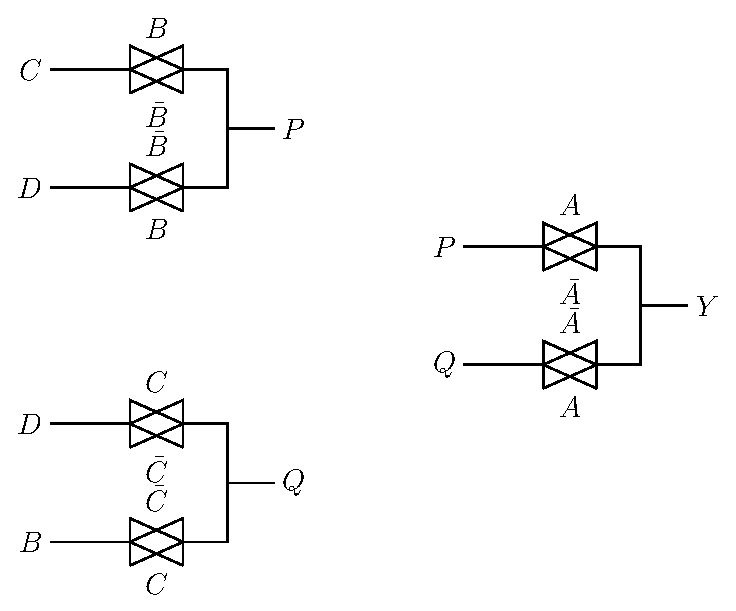
\includegraphics[width=.95\linewidth,height=.36\textheight,keepaspectratio]{Zadatak_10/kolo}
\caption{Tri multiplekserske grupe realizovane transmisionim gejtovima.}\label{fig:10.1}
\end{figure}
\subsection*{Rešenje}
\paragraph{a) Binarni ulazi.}
Gornja grana daje $P=\bar BD+BC$, a donja $Q=CD+\bar CB$. Izlaz bira $P$ za $A=1$, odnosno $Q$ za $A=0$:
\begin{equation}\label{eq:10.1}
Y=A(\bar BD+BC)+\bar A(CD+\bar CB)=A\bar BD+ABC+\bar ACD+\bar A\bar CB.
\end{equation}
\begin{table}[!htbp]\centering\caption{Funkcionalna tabela za binarne ulaze.}\label{tab:10.1}\begin{tabular}{cc}\toprule
$ABCD$ & $Y$\\
\midrule
\texttt{0000} & 0\\
\redlinija
\texttt{0001} & 0\\
\redlinija
\texttt{0010} & 0\\
\redlinija
\texttt{0011} & 1\\
\redlinija
\texttt{0100} & 1\\
\redlinija
\texttt{0101} & 1\\
\redlinija
\texttt{0110} & 0\\
\redlinija
\texttt{0111} & 1\\
\redlinija
\texttt{1000} & 0\\
\redlinija
\texttt{1001} & 1\\
\redlinija
\texttt{1010} & 0\\
\redlinija
\texttt{1011} & 1\\
\redlinija
\texttt{1100} & 0\\
\redlinija
\texttt{1101} & 0\\
\redlinija
\texttt{1110} & 1\\
\redlinija
\texttt{1111} & 1\\
\bottomrule\end{tabular}\end{table}
Za $ABCD=0101$ uključena donja grana bira $B=1$, pa je $Y=1$.
\paragraph{b) Visoka impedansa na ulazu D.}
TG prosleđuje odabrani ulaz, uključujući stanje $Z$ visoke impedanse. Ono nije treća logička vrednost na koju se neposredno primenjuje Bulova algebra. Tabela~\ref{tab:10.2} važi za $D\in\{0,1,Z\}$; kada piše $D$, izlaz prati baš taj ulaz. Za $D=Z$ nema aktivnog izvora koji garantuje napon izlaza, iako kapacitivnost može privremeno zadržati prethodni napon.
\begin{table}[!htbp]\centering\caption{Izlaz kada D može biti i visoke impedanse.}\label{tab:10.2}\begin{tabular}{cc}\toprule
$ABC$ & $Y$\\
\midrule
000 & 0\\
\redlinija
001 & $D$\\
\redlinija
010 & 1\\
\redlinija
011 & $D$\\
\redlinija
100 & $D$\\
\redlinija
101 & $D$\\
\redlinija
110 & 0\\
\redlinija
111 & 1\\
\bottomrule\end{tabular}\end{table}
\paragraph{c) Sinteza funkcije.}
Šenonovo razlaganje po A, pa B, daje
\begin{equation}\label{eq:10.2}
Y=AC+BC=A(C+BC)+\bar A(BC)=AC+\bar A[BC+\bar B\cdot0].
\end{equation}

Alternativno, razlaganje po C, pa A, daje
\begin{equation}\label{eq:10.3}
Y=C(A+B)+\bar C\cdot0=C[A\cdot1+\bar A B]+\bar C\cdot0.
\end{equation}

Prva realizacija je prikazana na slici~\ref{fig:10.2}. Četiri TG daju osam MOS tranzistora, ne računajući eventualne invertore za dobijanje komplementarnih upravljačkih signala.
\begin{figure}[!htbp]\centering
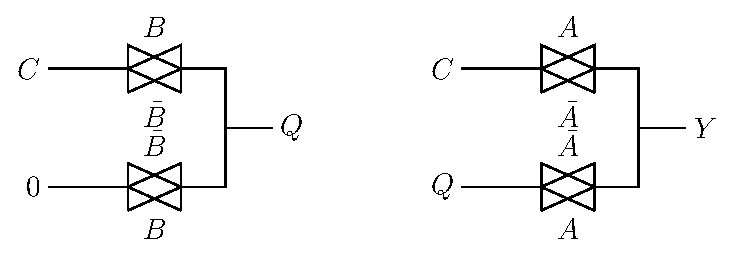
\includegraphics[width=.95\linewidth,height=.36\textheight,keepaspectratio]{Zadatak_10/sinteza}
\caption{TG realizacija funkcije Y=AC+BC prema prvom razlaganju.}\label{fig:10.2}
\end{figure}

\end{document}
